\documentclass[tikz,border=2pt]{standalone}

\usepackage[T1]{fontenc}
\usepackage{lmodern}
\usepackage{amsmath,amssymb}
\usepackage{xcolor}
\usepackage{tikz}
\usetikzlibrary{
  arrows.meta,
  backgrounds,
  calc,
  decorations.pathreplacing,
  fit,
  positioning,
  shapes.geometric
}

\definecolor{paperBlue}{HTML}{2F5E8C}
\definecolor{paperSky}{HTML}{E8F1F8}
\definecolor{paperGreen}{HTML}{2C7A5B}
\definecolor{paperMint}{HTML}{E7F3EE}
\definecolor{paperOrange}{HTML}{B86B18}
\definecolor{paperAmber}{HTML}{FFF0D8}
\definecolor{paperGray}{HTML}{4B5563}
\definecolor{paperLine}{HTML}{263238}

\begin{document}
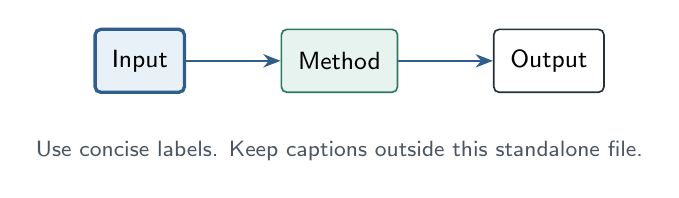
\begin{tikzpicture}[
  font=\sffamily\small,
  node distance=8mm and 12mm,
  box/.style={
    draw=paperLine,
    rounded corners=2pt,
    line width=0.6pt,
    fill=white,
    align=center,
    inner xsep=6pt,
    inner ysep=5pt,
    minimum height=8mm
  },
  primary/.style={box, draw=paperBlue, fill=paperSky, very thick},
  accent/.style={box, draw=paperGreen, fill=paperMint},
  note/.style={
    align=left,
    font=\sffamily\footnotesize,
    text=paperGray,
    inner sep=3pt
  },
  arrow/.style={
    -{Stealth[length=2.2mm,width=1.7mm]},
    line width=0.7pt,
    draw=paperLine,
    rounded corners=3pt
  },
  flow/.style={arrow, draw=paperBlue},
  feedback/.style={arrow, dashed, draw=paperOrange},
  zone/.style={
    draw=paperGray!35,
    rounded corners=4pt,
    dashed,
    fill=paperGray!5,
    inner sep=6pt
  }
]

% Replace this scaffold with the reconstructed paper figure.
\node[primary] (input) {Input};
\node[accent, right=of input] (method) {Method};
\node[box, right=of method] (output) {Output};

\draw[flow] (input.east) -- (method.west);
\draw[flow] (method.east) -- (output.west);

\node[note, below=5mm of method] {Use concise labels. Keep captions outside this standalone file.};

\end{tikzpicture}
\end{document}

